\documentclass{article}


\usepackage[margin=0.6in]{geometry}
\usepackage{amssymb, amsmath, amsfonts}
\usepackage{mathtools}
\usepackage{physics}
\usepackage{enumerate}
\usepackage{array}
\usepackage{tikz}
\usepackage{pgfplots}
\newcommand{\Rl}{\mathbb{R}}
\newcommand{\E}{\varepsilon}
\newcommand{\f}[3]{#1\ :\ #2 \rightarrow #3}

\title{MAT 228A Notes}
\author{Sam Fleischer}
\date{September 22, 2016}

\begin{document}
    \maketitle

    \section{Introduction}

        In MAT 228 we will study standard model PDEs, namely:
        \begin{enumerate}
            \item The Avection Equation (the typical hyperbolic equation)
            \begin{align*}
                u_t + c u_x = 0
            \end{align*}
            \item The Diffusion (Heat) Equation (the typical parabolic equation)
            \begin{align*}
                u_t = D u_{xx}
            \end{align*}
            \item The Poisson Equation (the typical elliptic equation)
            \begin{align*}
                u_{xx} = F
            \end{align*}
        \end{enumerate}

    \section{What we will not focus on in 228A}
        \subsection{The Avection Equation}

            Set $c \equiv 1$, and the domain $x > 0$.  Let the boundary condition be $u(0, t) = 1$ and the Initial condition
            \begin{align*}
                u(x,0) = f(x) \coloneqq \begin{cases}
                    1 & \text{if}\ 0 \leq x < \frac{1}{2} \\ 0 & \text{if}\ x \geq \frac{1}{2}
                \end{cases}
            \end{align*}

            Then for $t \geq 0$, the solution is
            \begin{align*}
                u(t,x) = \begin{cases}
                    1 & \text{if}\ 0 \leq x < t + \frac{1}{2} \\
                    0 & \text{else}
                \end{cases}
            \end{align*}
            that is, the wave transports to the right.

            \begin{center}
                \begin{tikzpicture}
                    \begin{axis}[legend pos=north east]
                        \addplot[domain=0:0.5,blue] {1};
                        \addplot[domain=0.5:5,blue] {0};
                        \draw[blue] (axis cs:0.5,1) -- (axis cs:0.5,0);
                        \legend{$t=0$}
                    \end{axis}
                \end{tikzpicture}
                \hspace{1cm}
                \begin{tikzpicture}
                    \begin{axis}[legend pos=north east]
                        \addplot[domain=0:2.7,blue] {1};
                        \addplot[domain=2.7:5,blue] {0};
                        \draw[->] (axis cs:2.4, .5) -- (axis cs:3, .5);
                        \draw[blue] (axis cs:2.7,1) -- (axis cs:2.7,0);
                        \legend{$t>0$}
                    \end{axis}
                \end{tikzpicture}
            \end{center}

        \subsection{The Heat Equation}

            Set $D \equiv 1$, and the domain $0 \leq x \leq 1$.  Set the boundary conditions:
            \begin{align*}
                u(0, t) = 1 \qquad u(1, t) = 0
            \end{align*}
            and initial condition $f(x)$ defined above.
            Then the discontinuity instantaneously smooths out so that $u(t,x) \in C^\infty$ for all $t > 0$, and the equilibrium state is stable and linear.
            \begin{center}
                \begin{tikzpicture}
                    \begin{axis}[legend pos=north east]
                        \addplot[domain=0:0.5, blue] {1};
                        \addplot[domain=0.5:1, blue] {0};
                        \draw[blue] (axis cs:0.5,1) -- (axis cs:0.5,0);
                        \legend{$t=0$}
                    \end{axis}
                \end{tikzpicture}
                \hspace{1cm}
                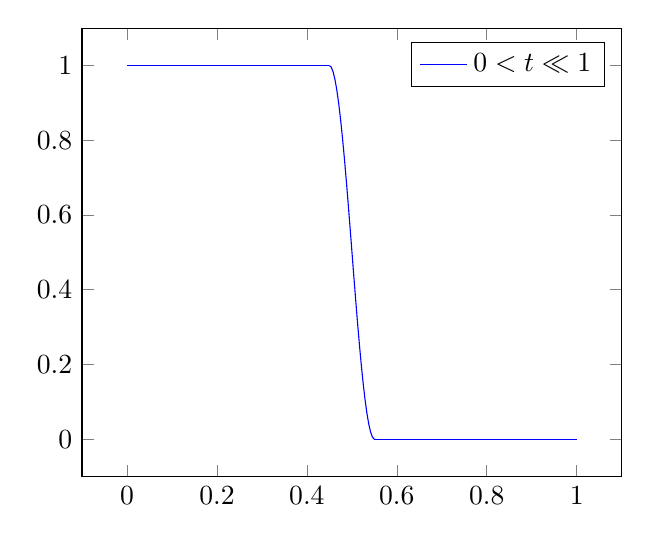
\begin{tikzpicture}
                    \begin{axis}[legend pos=north east]
                        \addplot[domain=0:0.45, blue] {1};
                        \addplot[domain=0.55:1, blue] {0};
                        \addplot[domain=0.45:0.55, blue] {0.5*cos(deg((1/0.032)*(x-.45)))+0.5};
                        \legend{$0 < t \ll 1$}
                    \end{axis}
                \end{tikzpicture}
            \end{center}
            \begin{center}
                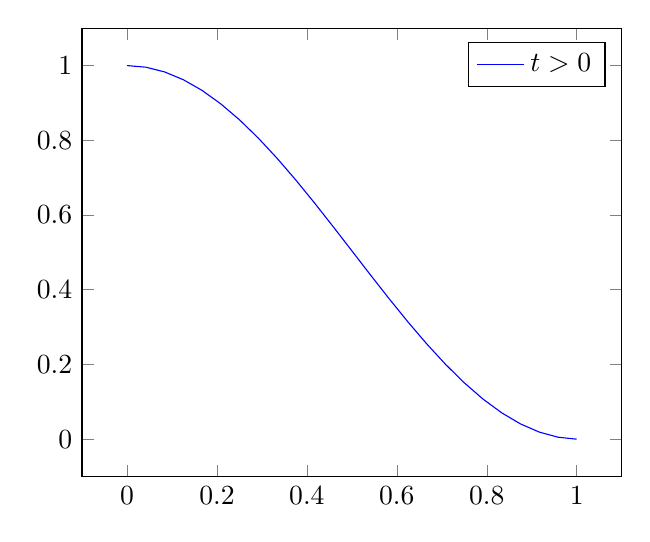
\begin{tikzpicture}
                    \begin{axis}[legend pos=north east]
                        \addplot[domain=0:1, blue] {0.5*cos(deg((1/0.32)*x))+0.5};
                        \legend{$t > 0$}
                    \end{axis}
                \end{tikzpicture}
                \hspace{1cm}
                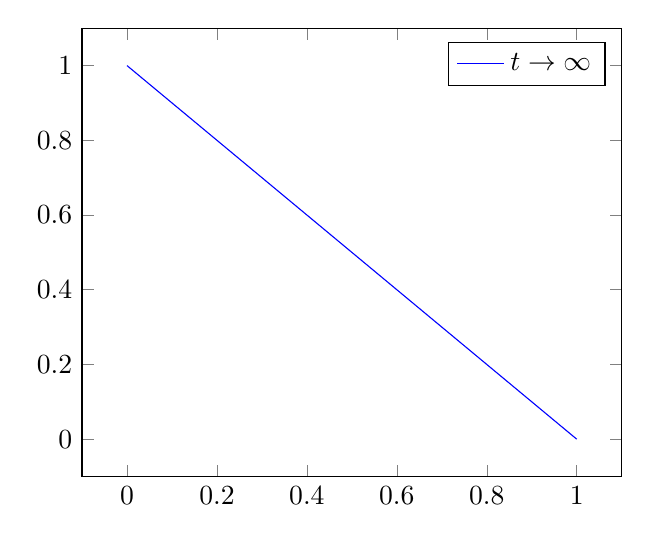
\begin{tikzpicture}
                    \begin{axis}[legend pos=north east]
                        \addplot[domain=0:1, blue] {1-x};
                        \legend{$t\rightarrow\infty$}
                    \end{axis}
                \end{tikzpicture}
            \end{center}

    \section{What we will focus on in 228A}

        We are focusing on the odd one out - it is time-independent.  Where do Poisson Equations show up?
        \begin{itemize}
            \item Steady State Diffusion Problems $(u_t = 0)$
            \begin{itemize}
                \item $u$ is a concentration
                \item $u_t = \underbrace{D u_{xx}}_{\text{transport by diffusion}} + \underbrace{F}_{\text{input}}$
                \item At steady state, $u_t = 0$, and so $-Du_{xx} = F$.
                \item $u_t = D u_{xx} \underbrace{- ku}_{\text{loss due to environment$\dots$causes exponential decay}} + f$
                \item At steady state, $-D u_{xx} + ku = f$, which is a Helmholtz Equation.
            \end{itemize}
            \item Electrostatics
            \begin{itemize}
                \item $\E$ is a steady electric field
                \item $\rho$ is a charge distribution
                \item $\E_0$ is a parameter
                \item $\grad\cdot \E = \frac{\rho}{\E_0}$
                \item Given the charge distribution, we want to find the electric field.
                \item $\underbrace{\grad \times \E}_{\text{curl}} = 0\ \implies\ \exists$ potential function $\phi$ such that $\E = -\grad\phi$.
                \item So, $\grad \cdot \E = \grad(-\grad\phi) = \underbrace{-\Delta \phi = \frac{\rho}{\E_0}}_{\text{Poisson Equation}}$
            \end{itemize}
            \item Potential Flow
            \begin{itemize}
                \item $\grad u = 0$, where $u$ is velocity.  $\grad u = 0$ means it is divergence-free, and thus incompressible.
                \item With high Reynolds number it is curl-free, and thus there is a potential function $\phi$ such that $\Delta\phi = 0$, which is a Poisson equation.
                \item With low Reynolds number (usually on very small length scales, i.e.~bacterial swimming), it is drag-dominated, effectively no inertia.
                \item We have $\mu\Delta u - \grad p = 0$, so $\grad \cdot u = 0$, which implies it is imcompressible.  These are Stokes Equations.
                \item Take Divergence, and assume commutativity with the Laplacian $\Delta$, and thus $-\Delta p = 0$, which is a Poisson Equation.
            \end{itemize}
        \end{itemize}

        The Poisson equation is
        \begin{align*}
            u_{xx} &= f & \text{in one dimension} \\
            u_{xx} + u_{yy} &= f & \text{in two dimensions in the Cartesian coordinates} \\
            \Delta u &= f\ \ \text{or}\ \ (\grad \cdot \grad) u = f\ \ \text{or}\ \ \grad^2 u = f & \text{in any number of dimensions (finite)}
        \end{align*}
        These equations need a defined domain and boundary conditions.

        \subsection{1-Dimensional Diffusion Equation}
            Consider a long thin metal tube, which can be represented as a function in one dimension.  Let $u(x,t) \coloneqq $ the concentration of some chemical (or heat, or whatever) at time $t$ and position on the tube $x$, where $x \in [a,b]$.  Then
            \begin{align*}
                u_t = D u_{xx} + F
            \end{align*}
            What can the boundary conditions be?  The easiest condition is to hook one side up to a giant vat with constant concentration so that $u(0,t) = u_0$ is constant, which is called Dirichlet Boundary Condition.

            The second type of condition is called a Neumann Boundary Condition, which is a condition on the flux at the boundary.  For example, we could cap one end so that no transport can happen through the boundary.  Given $(a,b)$, define
            \begin{align*}
                q(t) \coloneqq \int_a^b u(x,t)\dd x \qquad \text{(this is the total amount of chemical in the interval $(a,b)$ at time $t$)}
            \end{align*}
            So,
            \begin{align*}
                u_t &= D u_{xx} \\
                \implies \int_a^b u_t \dd x &= \int_a^b D u_{xx} \dd x \\
                \implies \frac{\dd}{\dd t} q(t) &= \underbrace{D\qty[u_x(b,t) - u_x(a,t)]}_{\text{these terms describe tre transport rate on the boundary}}
            \end{align*}
            Define $J \coloneqq -Du_x$ as the diffusive flux.  So if we want no flux (which is the only means of transport), we must have $u_x(0,t) = 0$.  Or, given some constant injection on an end point, we could set
            \begin{align*}
                -D u_x(0,t) = g, \qquad \text{where $g$ is constant.}
            \end{align*}

            The last type of condition can be likened to a semi-permeable membrane on the boundary.  It is called a Robin Boundary Condition, and is simply a linear combination of Dirichlet and Neumann conditions.  So,
            \begin{align*}
                J = \alpha(u_r - u_\ell)
            \end{align*}
            The flux balances so that
            \begin{align*}
                -D u_x(0,t) = \alpha(u(0,t) - u_0)
            \end{align*}
            and thus
            \begin{align*}
                \alpha u(0,t) + D u_x(0,t) = \alpha u_0.
            \end{align*}

\end{document}